\documentclass[tikz]{standalone}

\usepackage{fp}
\usepackage{tikz}
\usepackage{tikz-3dplot}
\usepackage{amsmath} %математические формулы
\usepackage[e]{esvect}  %Красивая стрелочка вектора


\usetikzlibrary{calc}
\usetikzlibrary{arrows.meta}

\begin{document}
	

	
	
	
	 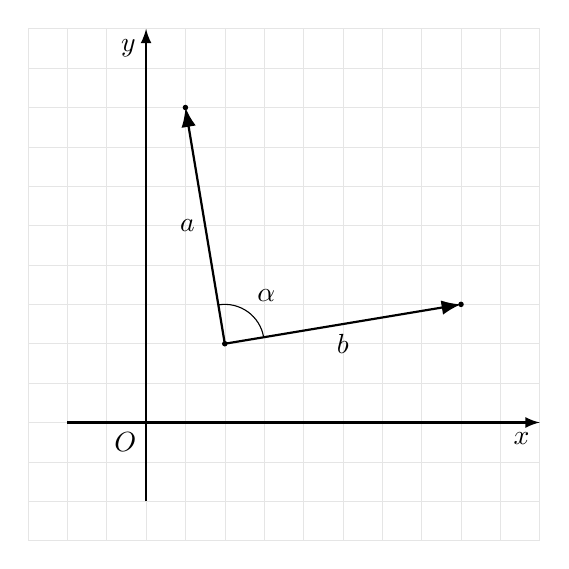
\begin{tikzpicture}[scale=1]
		
		
		\draw[step=.5cm,black!10,very thin] (-1.5,-1.5) grid (5,5);
		
		\draw[-latex, thick] (-1,0) -- (5,0) node [below left] {$x$};
		\draw[-latex, thick] (0,-1) -- (0,5) node [below left] {$y$};
		
		\coordinate (O) at (0,0);
		
		\draw (O) node [below left] {$O$};
		
		
		\coordinate (A) at (1,1);
		\coordinate (B) at (0.5,4);
		\coordinate (C) at (4,1.5);
		
		
		
		\fill [black] (A) circle [radius=1pt];
		\fill [black] (B) circle [radius=1pt];
		\fill [black] (C) circle [radius=1pt];
		
		
		
		
		\draw[-{Latex[length=7pt]}, thick] (A) -- (B) node [left, midway] {$\vv{a}$};
		\draw[-{Latex[length=7pt]}, thick] (A) -- (C) node [below, midway] {$\vv{b}$};
		
		\draw ($(A) + ({atan2(1,6)}:0.5cm)$) arc ({atan2(1,6)}:{atan2(6,-1)}:0.5cm) node [above right, midway] {$\alpha$};
		

		
		
	\end{tikzpicture}
		

	
\end{document}